\section{Project 1 - 交叉线}

\subsection{搜索算法的设计思路}

对于交叉线问题, 我们令初始状态的各个点定义为可移动的点, 让这些点在棋盘上游走, 其经过的
轨迹会留下相应的颜色, 每个格子额外记录从上一个格子移动向本个格子的移动方向(用于计算转向惩罚); 因此状态
空间即为所有格子的颜色, 方向, 是否可移动三个属性的状态空间的积. 如果一个可移动的点
尝试向另一个同色的可移动的点进行移动, 这种颜色的线连接完成, 将二者均从可移动的点的集合
中删去. 如果可移动的点集合为空, 则说明达到了目标状态.

启发函数可以在以下三种中选择(括号内为在图形界面中显示的名字):

\begin{enumerate}
    \item $0$启发函数. (Null Value Function)
    \item 所有可移动的点的曼哈顿距离之和 (Manhattan Distance)
    \item 在第二个的基础上, 对于每一对可移动的点, 若不在一行且不在一列, 则令代价额外加$2$. (Manhattan with Penalty)
\end{enumerate}

实现的搜索算法为A*算法.

\subsection{搜索算法的结果演示}

部分示例的结果如图\ref{fig:proj1-1}所示. 对于示例$1$, 打开惩罚和关闭惩罚搜索得到的结果不同,
可见A*算法确实能够根据不同的问题条件完成不同的结果搜索. 示例2是问题给出的示例, 可见对于较为复杂的交叉线
问题其也可以给出答案.

\begin{figure*}
    \centering
    \subfigure[示例1-无惩罚]{
        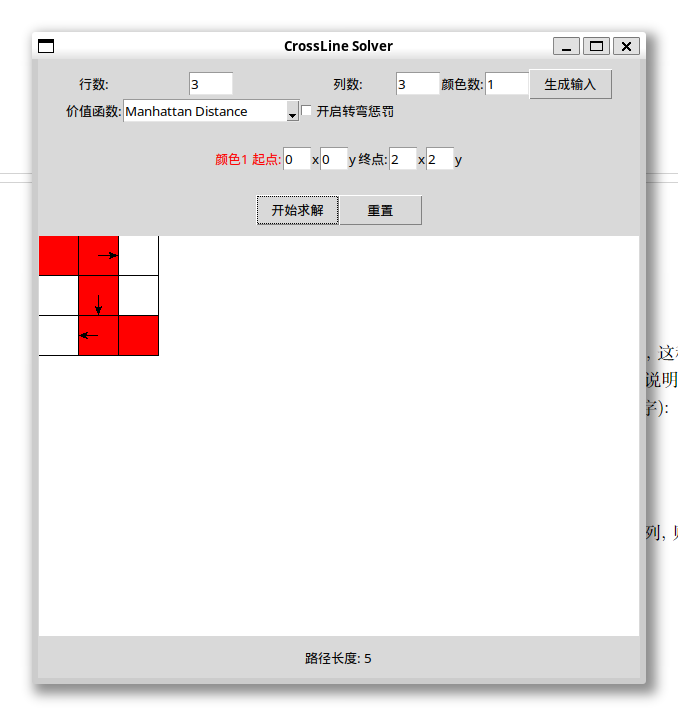
\includegraphics[width=0.4\textwidth]{images/no-penalty.png}
    }
    \subfigure[示例1-有惩罚]{
        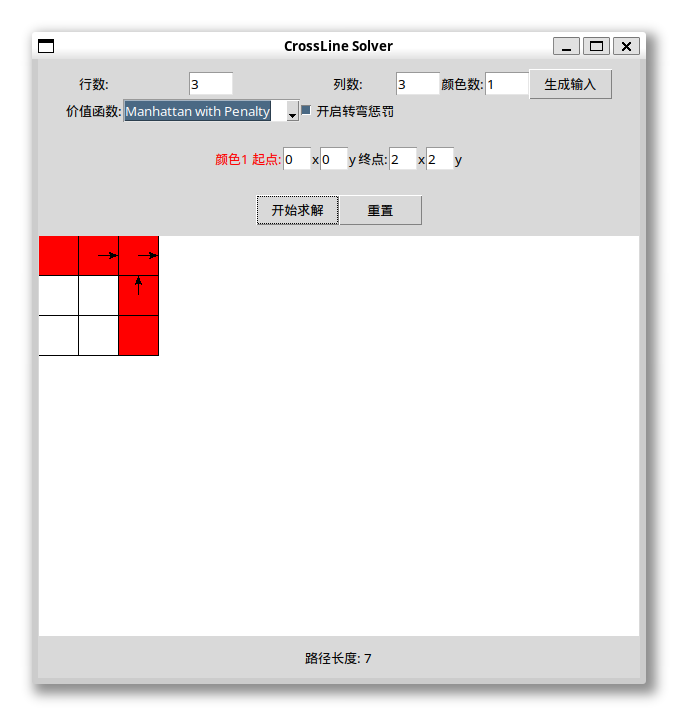
\includegraphics[width=0.4\textwidth]{images/with-penalty.png}
    }
    \subfigure[示例2-无惩罚]{
        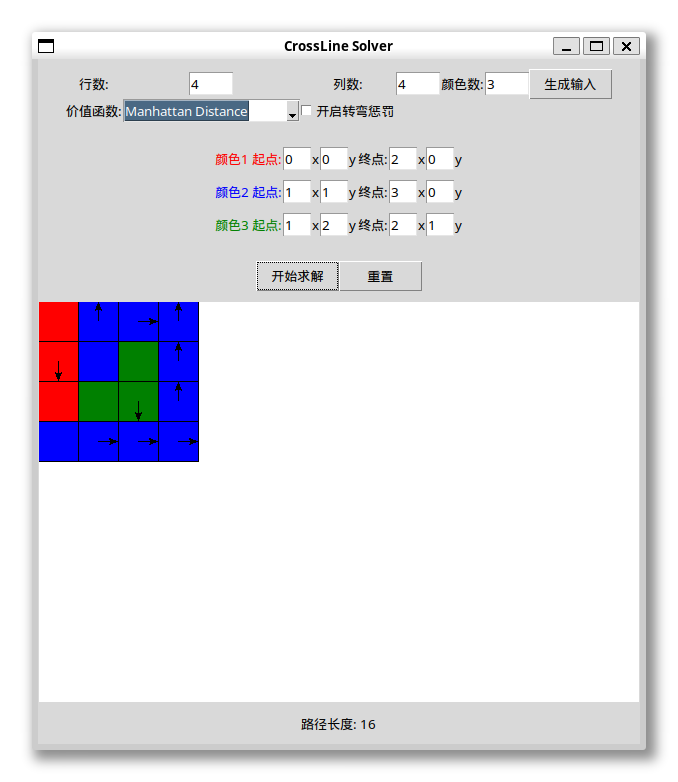
\includegraphics[width=0.4\textwidth]{images/no-penalty-2.png}
    }
    \subfigure[示例2-有惩罚]{
        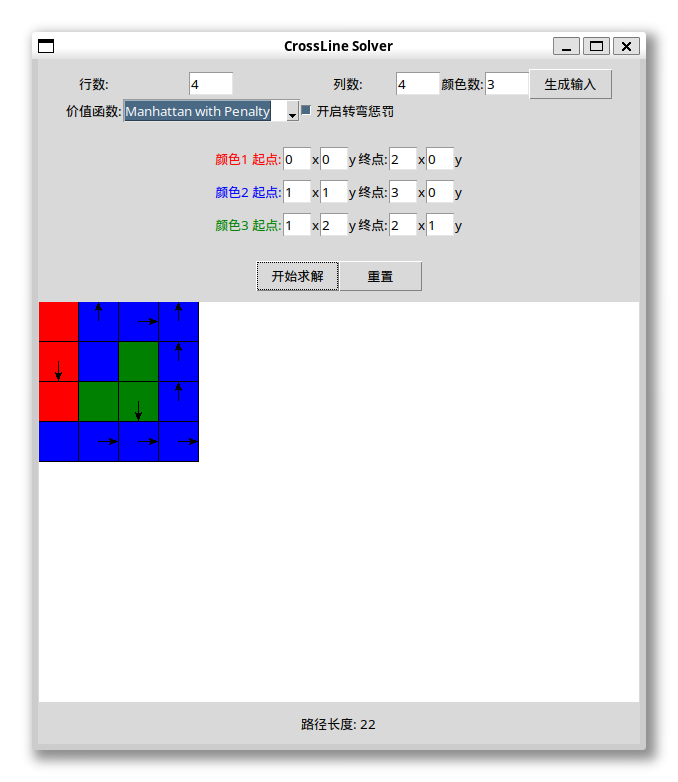
\includegraphics[width=0.4\textwidth]{images/with-penalty-2.png}
    }
    \caption{交叉线算法结果}\label{fig:proj1-1}
\end{figure*}

\subsection{必要的讨论}

调试过程中的问题主要集中在对于状态的定义上; 一开始对于状态的定义是对于每个格子只比较其颜色,
如果每个格子的颜色均相同则认为状态相同; 这样定义无论怎样搜索都是无解, 因为当两个同色可移动点相遇时,
所作的操作仅仅是将这两个可移动点标记去除, 并未改变棋盘颜色, 因此当搜索到这种状态时, 搜索算法会认为
其已经在\verb|closed_list|中而将其丢弃.

正确的定义是为每一个可移动点定义一个唯一编号, 在比较格子时不仅要比较格子是否可移动, 还要比较
每个可移动格子的编号是否相等, 否则也应该认为是不同状态(例如蓝色的两个可移动点相比较时应当认为是不同).
